\documentclass{sig-alternate}

\usepackage{graphicx} 
\usepackage{subfigure}
\usepackage{paralist}
\usepackage[]{algorithm2e}
\usepackage{hyperref}

\usepackage{url}
\usepackage{booktabs}

\usepackage[usenames,dvipsnames]{xcolor}
\usepackage{tikz}
\usetikzlibrary{positioning, calc}

\usepackage[draft,nomargin,footnote]{fixme}

\graphicspath{{figs/}}

\usepackage{xspace}
\newcommand{\eg}{\textit{e.g.}\xspace}
\newcommand{\etal}{\textit{et al.}\xspace}
\newcommand{\ie}{\textit{i.e.}\xspace}
\newcommand{\etc}{\textit{etc.}\xspace}
\newcommand{\vs}{\textit{vs.}\xspace}

\begin{document}

% if need info about conference :
%\conferenceinfo{WOODSTOCK}{'97 El Paso, Texas USA}

\title{Building successful long child-robot interactions in a learning context}
\conferenceinfo{HRI}{'16 Chrischurch, New Zealand.}

\author{Alexis Jacq$^{1,2}$, S\'everin Lemaignan$^1$, Fernando Garcia$^1$, Pierre Dillenbourg$^1$, Ana Paiva$^2$\\
$^1$CHILI Lab, \'Ecole Polytechnique F\'ed\'erale de Lausanne, Switzerland,\\
$^2$Instituto Superior T\'{e}cnico, University of Lisbon, Portugal}


%   \author{
%   % 1st. author
%   \alignauthor
%   Alexis Jacq\\
%       \affaddr{EPFL}\\
%       \affaddr{IST}
%   % 2nd. author
%   \alignauthor
%   Severin Lemaignan\\
%       \affaddr{EPFL}
%   \and
%   % 3rd. author
%   \alignauthor Fernando Garcia\\
%       \affaddr{EPFL}
%
%   \alignauthor Pierre Dillembourg\\
%       \affaddr{EPFL}
%
%   \alignauthor Ana Paiva\\
%           \affaddr{IST}
%    }


\maketitle
\begin{abstract}

The CoWriter activity involves a child in a rich and complex interaction where he has to
teach handwriting to a robot. The robot must convince the child it needs his help and it
actually learns from his lessons. To keep the child engaged, 
the robot must learn at the right rate, not too fast otherwise the kid will have
no opportunity for improving his skills and not too slow otherwise he may loose
trust in his ability to improve the robot' sills.
We tested this approach in real pedagogic/therapeutic contexts with
children in difficulty over repetitive long sessions (40-60 min). Through 3 different
case studies, we explored and refined experimental designs and algorithms in order to fit
troubles of each child and to promote their motivation and self-confidence. We report positive observations, suggesting an intrinsic engagement of children to help the
robot, and their comprehension that they were good enough to be teachers, while they cam with
a feeling of handicap in handwriting. 

\end{abstract}

%\keywords{child-robot interaction, learning by teaching, protégé effect, children self-confidence, intrinsic motivation, robotic handwriting learning}

\section{Introduction}

Children facing difficulties in handwriting integration are more exposed
to troubles during the acquisition of other disciplines as they grow up
\cite{Christensen2005}. 
The Cowriter activity introduces a new approach to help those children
\cite{Hood}. While common successful interventions involve children
in long intervention (at least 10 weeks) focused on \emph{motor} skills \cite{Hoy2011},
CoWriter is based on \emph{learning by teaching} paradigm and aims to repair
self-confidence and motivation of the child rather than his handwriting performance alone.

\emph{Learning by teaching} is a technique that engages students to conduct the activity in the role of the teachers in order to support their learning process. This 
paradigm is known to produce motivational, meta-cognitive and educational
benefits in a range of disciplines~\cite{Rohrbeck2003}. The CoWriter project
is the first application of learning by teaching approach to handwriting. 

The effectiveness of our learning by teaching activity is build on the
``prot\'eg\'e effect'': the teacher feels responsible for his student, commits
to the student's success and possibly experiences student's failure as his own
failure to teach. Teachable computer-based agents have previously been used to
encourage this ``prot\'eg\'e effect'', where students invest more effort into
learning when it is for the benefit of a teachable agent than for themselves~\cite{Chase2009}.
We rely on this cognitive mechanism to reinforce the child's commitment into the
robot-mediated handwriting activity.

In this study, we assume that the key of such a relationship between the child
and the robot relies on the credibility of the robot:
The more the robot convinces the child that it is a beginner in
handwriting who needs help -- building the ``prot\'eg\'e effect''-- the better
the child will engage in the interaction. Two important technical aspects of
credibility are: how to generate the initial state of the robot, and how to design its
learning behavior. In our previous work, we used a limited approach in which
letters had to be written as a single stroke (no pen lifting) and that covered
typical mistakes of adults extracted from an handwritten letters database. Experiments with CoWriter were conducted in school, involving either group of
children doing the activity together or children
in short individual sessions.

These studies have been conducted to evaluate the feasibility and technical soundness
of the interaction system. Because of the group effect and the briefness of
interactions, no conclusions were reached about any positive effect of the
interaction. Subject children where randomly chosen in school
classes and had no specific difficulties in handwriting. This made it
impossible to observe any remediation of self-esteem or motivation.

In this paper, we explore different algorithmic and staging approaches built on the system presented in~\cite{hood2015when} in order to figure out intricate aspects of long child-robot interactions in a pedagogical context. We solved previous 
technical limitations of robot's letter learning and generation, and we introduce new algorithmic approaches that make robot's behaviour more convincing.
Through three experiments, we involved children with real difficulties or low 
self-esteem in repeated long sessions (four times about one hour). We used different
measures, both qualitative and quantitative, to express the impact of those
interaction with the CoWriter robot on the child.

This article consists of four sections. In the first section we give technical details of our setup, such as how are connected the different modules
together and which algorithms are used to learn and generate robot's letters.
The following three parts report our three experiments and results. Two case studies specifically designed to be adapted to one child; one introduces a general design conducted with 8 children separately. 


\section{related works}

Robots have already been used as a social partner in educational
contexts. Lots of studies have been conduced with language skills
acquisition~\cite{han2010robot}, less often involving physical skills (such as
calligraphy~\cite{Matsui2013}). Regarding \textit{learning by teaching} paradigm with
robots, Werfel notes in~\cite{Werfel2014} that studies tend to focus on the
ability of the robots to learn (in terms of language~\cite{Saunders2010} or
physical~\cite{Mulling2013} skills, for example) rather than the beneficial impact
on the teaching for the human. To contrary, our work minimized the robot's skills while we
concentrate on the possible improvement of children self-confidence and
motivation promoted by the behaviour of the robot.

%   \begin{figure}
%       \centering
%       \includegraphics[width=0.9\linewidth]{Thomas}
%       \caption{Thomas teaching Nao how to write numbers, with the help of an occupational therapist.}
%       \label{fig:Thomas}
%   \end{figure}

\section{Experiments design}
\subsection{Interaction overview}
Figure~\ref{experimental_setup} illustrates our general experimental setup: a
face-to-face child-robot interaction with an (autonomous) Aldebaran's {\sc nao}
robot.

A tactile tablet (with a custom application) is used by both the robot and the
child to write: in each turn, the child requests the robot to write
something (a single letter, a number or a full word), and pushes the tablet
towards the robot, the robot writes on the tablet by gesturing the writing (but
without actually physically touching the tablet). The child then pulls back the
tablet, corrects the robot's attempt by writing himself on top or next to
the robot's writing (see Figure~\ref{fig:Vincent}), and ``sends'' his
demonstration to the robot by pressing a small button on the tablet. The robot
learns from this demonstration and tries again.

Since the child is assumed to take on the role of the teacher, we had to ensure
he would be able to manage by himself the turn-taking and the overall
progression of the activity (moving to the next letter or word). In our design,
the turn-taking relies on the robot prompting for feedback once it is done with
its writing (simple sentences like ``What do you think?''), and pressing on a
small robot icon on the tablet once the child has finished correcting. We found that both approaches were easy to grasp for children.


   \begin{figure}
       \centering
       
\includegraphics[width=0.6\columnwidth]{experimental_setup}
       \caption{\small Our experimental setup: face-to-face interaction with a {\sc
           nao} robot.  The robot writes on the tactile tablet, the child then
           corrects the robot by directly overwriting its letters on the tablet
           with a stylus. An adult (either a therapist or an experimenter,
           depending on the studies), remains next to the child to guide the work
           (prompting, turn taking, etc.). For some studies, a second tablet and an
           additional camera (lightened) are employed.}

       \label{experimental_setup}
   \end{figure}

\subsection{Generating and learning letters}
Since our approach is based on teaching a robot to write, generating (initially
bad) letters and learning from demonstrations is a core aspect of the project.
The initial state of the robot and his ability to learn in an obvious way
from demonstrations of the child is the key to lend credibility to the activity and to induce the ``prot\'eg\'e" effect.

The technical idea is simple: allographs of letters are encoded as a sequence of 70 points in
2D-space and can be seen as vectors with 140 elements
($x_1,...,x_{70},\hspace{1mm}y_1,...,y_{70}$). We arbitrary chose a set of allograph
that define the initial state of generated letters. 
After the child provided a demonstration of a letter, the algorithm
generates a new letter corresponding to the middle point between the last state and the
demonstration. 

In the following sections, we present various techniques to
create the initial state, and different metrics used to compute progression of the robot, tested as hypothesis within our three experiments. 

\subsubsection{Generation of initial allographs}
The first question relates to the construction of the initial set of allographs.
In previous experiments presented in~\cite{hood2015when}, we built a subspace based on principal component
analysis (PCA) of a standard dataset of 214 adult letters (the UJI Pen Characters 2 dataset~\cite{Llorens2008}).
We used the first $n$ eigenvectors (in
these experiments, $3 < n < 6$) of the covariance matrix
generated from PCA to create a subspace. To create new letter shapes, we chose
random coordinates close to the origin of this subspace. Each eigenvector
provided the direction of a principal deformation of the allograph in human
handwriting~\cite{Hood}. But generated ``imperfections" of letters were not representative of
children deformations: they were reflecting typical defects when adults are writing to fast. 
Over the following studies, we explored three different ways to generate samples closer to beginners. In our first case study (section~\ref{Vincent}), we used homework of the child previously provided
by his mother, to exaggerate by hand his main defects. This way, the child was
going to correct his own kind of mistakes. In the second study (section~\ref{Thomas}),
the child was suffering from visuo-constructive deficits. Since it was
difficult for him to improve already recognisable allographs, we decided under the
guidance of his occupational therapist to make the robot start from simple
vertical stroke for all letters. In
the third study~\ref{auto} we chose to use the middle point between a vertical stroke
and correct letters as a starting point for the robot. 

\subsubsection{Metrics used for the learning curve of the robot}
The second question focuses on the learning algorithm. In
~\cite{Hood}, we were projecting children's demonstrations in PCA's subspace in order to 
compute the middle between that point and the previous state of the robot. Then, we
generated the allograph in middle way as the new state of
the robot. For the experiments introduced in this paper, we explored two other
ideas: In the first study (section~\ref{Vincent}) we generated a PCA subspace from a
small set of allographs we drew arbitrary. Each time the child was providing a
demonstration, we added that demonstration to the small set and re-built the
PCA subspace. That way, the principal eigenvectors obtained progressively
tended to encode the main deformations of letter done by the child. The following algorithm explains the successive steps of this approach:

\begin{algorithm}
   generate initial dataset $D$\;
   generate initial subspace $S$ by PCA of $D$\;
   generate initial robot state $r$ (random point in $S$)\;
   \If{robot receives a demonstration $d$}{
   	add $d$ to dataset: $D'\leftarrow D\cup d$\;
   	recompute subspace $S'$ by PCA of $ D'$\;
   	compute coordinates $r'$ of $r$ in $S'$\;
   	compute coordinates $d'$ of $d$ in $S'$\;
   	learn the demonstration: $r''= \frac{1}{2} \dot (r'+d')$\;
   }
   \caption{learning from demonstration in adaptive PCA subspace}
\end{algorithm}

From our perspective, this dynamic subspace was more adapted to the 
progression of the child, and the sequence of tries performed by the robot looked smoother.
However using metrics in subspace can make the learning algorithm too slow in some
cases, because consecutive projected demonstrations can sometimes be too
far from each other in subspace while they appears similar in Cartesian space.
In other studies, we decided to put aside the PCA approach and to always use the middle point in Cartesian space, in order to
have a better control over the convergence of the robot tries to the demonstrations.


\subsection{robotic implementation}

The actual implementation on the robot requires the coordination of
several modules (from performing gestures and acquiring the user's input to
the high-level state machine), spread over several devices (the robot itself,
one laptop and up to four tactile tablets for certain studies we conducted). We
relied on ROS to ensure the synchronization and communication between different devices.

Our system is embodied in an Aldebaran's {\sc nao} (V4 or V5, depending on the
studies) humanoid robot. This choice is motivated by its approachable
design~\cite{Gouaillier2008}, its size (58cm) and inherently safe structure
(lightweight plastic) making it suitable for close interaction with children,
its low price (making it closer to what school may afford in the coming years)
and finally its ease of deployment on the field.

Robotic handwriting requires precise closed-loop control of the arm and hand
motion. Because of the limited fine motor skills possible with such an
affordable robot, in addition to the absence of force feedback, we have opted
for \emph{simulated handwriting}: the robot draws letters in the air, and the
actual writing is displayed on a synchronised tablet.

\begin{figure}[ht!]
\centering

\resizebox{1.1\linewidth}{!}{%

\begin{tikzpicture}[
    >=latex,
    node distance=2cm,
    every edge/.style={draw, very thick},
    redarrow/.style={draw,red, text=black},
    greenarrow/.style={draw,GreenYellow,text=black},
    yellowarrow/.style={draw,BurntOrange,text=black},
    cmpt/.style={draw, align=center, rounded corners, inner sep=5pt, font=\sf, fill=black!20},
    label/.style={midway, align=left, font=\scriptsize\sf, fill=white, above,opacity=0,text opacity=1}]

    \node at (0,0) (laptop) {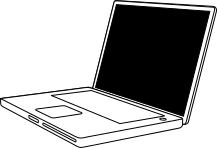
\includegraphics[width=2cm]{laptop}};
    \node[below right=2 of laptop] (nao) {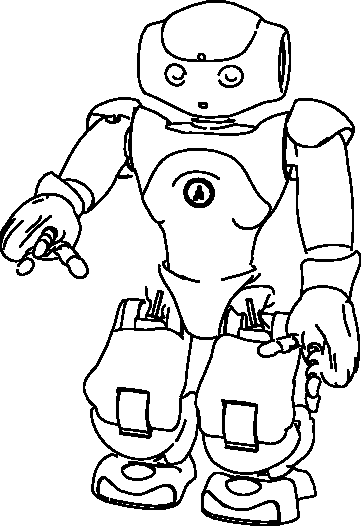
\includegraphics[width=2cm]{nao}};
    \node[below left=2 of laptop] (tablet) {
\includegraphics[width=2cm]{tablet+stylus}};
    \node[above=2 of laptop] (selection) {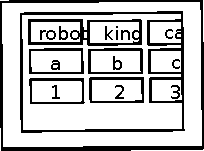
\includegraphics[width=2cm]{selection_tablet}};

    \node[draw,above right=2 of laptop,anchor=north west,text width=4cm] (processes)
    {\sf\scriptsize machine-learning, \\letters/gestures
    generation, \\interaction supervision};
    \path (laptop) edge[dashed] (processes);

    \path (nao) edge [->,redarrow, bend left] node[label, auto] {robot state} (laptop);
    \path (laptop) edge [->,greenarrow, bend left] node[label, auto] {writing gestures} (nao);

    \path (tablet) edge [->,redarrow, bend left] node[label, auto] {demonstrations,\\turn taking} (laptop);
    \path (laptop) edge [->,redarrow, bend left] node[label,
    auto=right,align=right]
    {path of\\ letters to display} (tablet);

    \path (selection) edge [->,redarrow] node[label, auto=right] {letter/word to write} (laptop);

    \path (-5, 2) edge [->, redarrow] node[label] {ROS} ++(1, 0);
    \path (-5, 2.6) edge [->, greenarrow] node[label] {NaoQI} ++(1, 0);
    
\end{tikzpicture}
}

\caption{\small \textbf{Overview of the system}. In total, the system runs about 10 ROS nodes,
    distributed over the robot itself, a central laptop and Android tablets.}

    \label{fig:archi}
\end{figure}

The overall architecture of the system (Figure~\ref{fig:archi}) is therefore
spread over several devices: the {\sc nao} robot itself, that we address via
both a ROS API\footnote{The ROS stack for {\sc nao} is available at 
\url{http://wiki.ros.org/nao_robot}.} and the Aldebaran-provided NaoQI API, one
to four Android tablets (the main tablet is used to print the robot's letter and
to acquire the children's demonstrations; more tablets have been used in some
studies, either to let the child input words to be written, or for the
experimenter to qualitatively annotate the interaction in a synchronized
fashion), and a central laptop running the machine learning algorithms, the
robot's handwriting gesture generation and high level control of the activity.

Since the system does not actually require any CPU-intensive process, the laptop
can be removed and the whole logic run on the robot. Due to the relative
difficulty to deploy and debug ROS nodes directly on the robot, the laptop
remains however convenient during the development phase and we kept using it in
our experiments.

Most of the nodes are written in Python, and the whole source code of the
project is available online\footnote{The primary repository is\\ 
\url{https://github.com/chili-epfl/cowriter_letter_learning}.}.


\section{case study 1: Vincent}\label{Vincent}
\subsection{Context}
Vincent is a five year-old child. At school, he had difficulties to learn writing, particularly with cursive letters. From our perspective, Vincent is shy and quiet. He suffers from poor self-confidence much more than any actual writing problem.

\subsection{Questions}

The CoWriter activity needs a child engaged as interaction leader. 
With this study we consider the problem of long-term interactions: is it possible to
sustain this engagement over several one-hour sessions?

%   \begin{figure}
%       \centering
%       \includegraphics[width=0.9\linewidth]{Vincent_start}
%       \caption{Homework performed by Vincent before the experiment. It gives an
%       overvew of his starting level in handwriting.}
%       \label{fig:Vincent_start}
%   \end{figure}
%
%   \begin{figure}
%       \centering
%       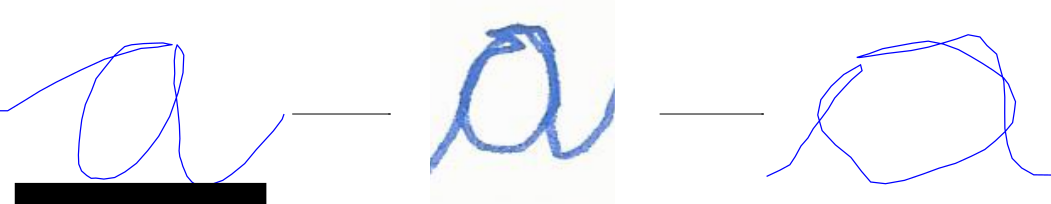
\includegraphics[width=0.9\linewidth]{3a}
%       \caption{Letter deformation along an eigenvector. \emph{Left} : the non-deformed
%           letter (origin of the subspace). \emph{Middle} : the actual Vincent's
%           deformation (from figure~\ref{fig:Vincent_start}). \emph{Right} : exaggerated
%   deformation along the eigenvector that encode Vincent's mistake.} 
%       \label{fig:3a}
%   \end{figure}

\subsection{Experimental settings}

The experiment as conducted in laboratory setting. Our goal was to provide Vincent with
an environment that would enable him to sustain engagement over four one-hour sessions, 
one session per week. We decided 
to introduce a scenario that justified the activity to the child
where a robot wants to learn handwriting. We used two Nao robots: a blue one 
(called Mimi) and an orange one (called Clem). Mimi was away for a 
scientific mission, and the two robots had to communicate by mails. But they decided to do it 
``like humans", with handwritten messages. While Mimi was good in handwriting, 
Clem had strong difficulties and needed Vincent's help.

Mimi's mission was to explore a mysterious hidden
base. Each week, a postal mail contenting
a picture of a curious object it found and a few handwritten words about its discoveries. 
The picture showed itself exploring 
a dark room of the hidden base (that was actually our laboratory's workshop). 

During the three first sessions, Clem (the robot interacting with the child) was waiting for Vincent
with the received mail. It let Vincent take a look at the picture and the object,
and then it asked him to read the message.
Finally, Vincent formulated a response and helped the robot to write it.

The fourth and last session was set as a test: Mimi, the ``explorer'' robot,
came back from its mission and challenged Clem in
front of Vincent: \emph{``I don't believe you wrote yourself these nice letters that I
received! Prove it to me by writing something in front of me!''} This situation
was meant to confirm the prot\'eg\'e effect: by judging the other robot's
handwriting, Mimi would implicitly judge Vincent's skills as
teacher, and in turn, Vincent's handwriting.

To complement the intrinsic motivation of helping a robot to communicate with another one, we
gradually increased the complexity of Vincent's task to keep it challenging and
interesting (first week: demonstration of single letters; second week:
short words; third week: a full message -- Figure~\ref{fig:stimuli}).

Vincent had to tell the robot what to write with small plastic letters (visible
behind the robot on Figure~\ref{fig:Vincent}). A third person was here to send
the formed word to the robot via the computer.

%   \begin{figure}
%       \centering
%       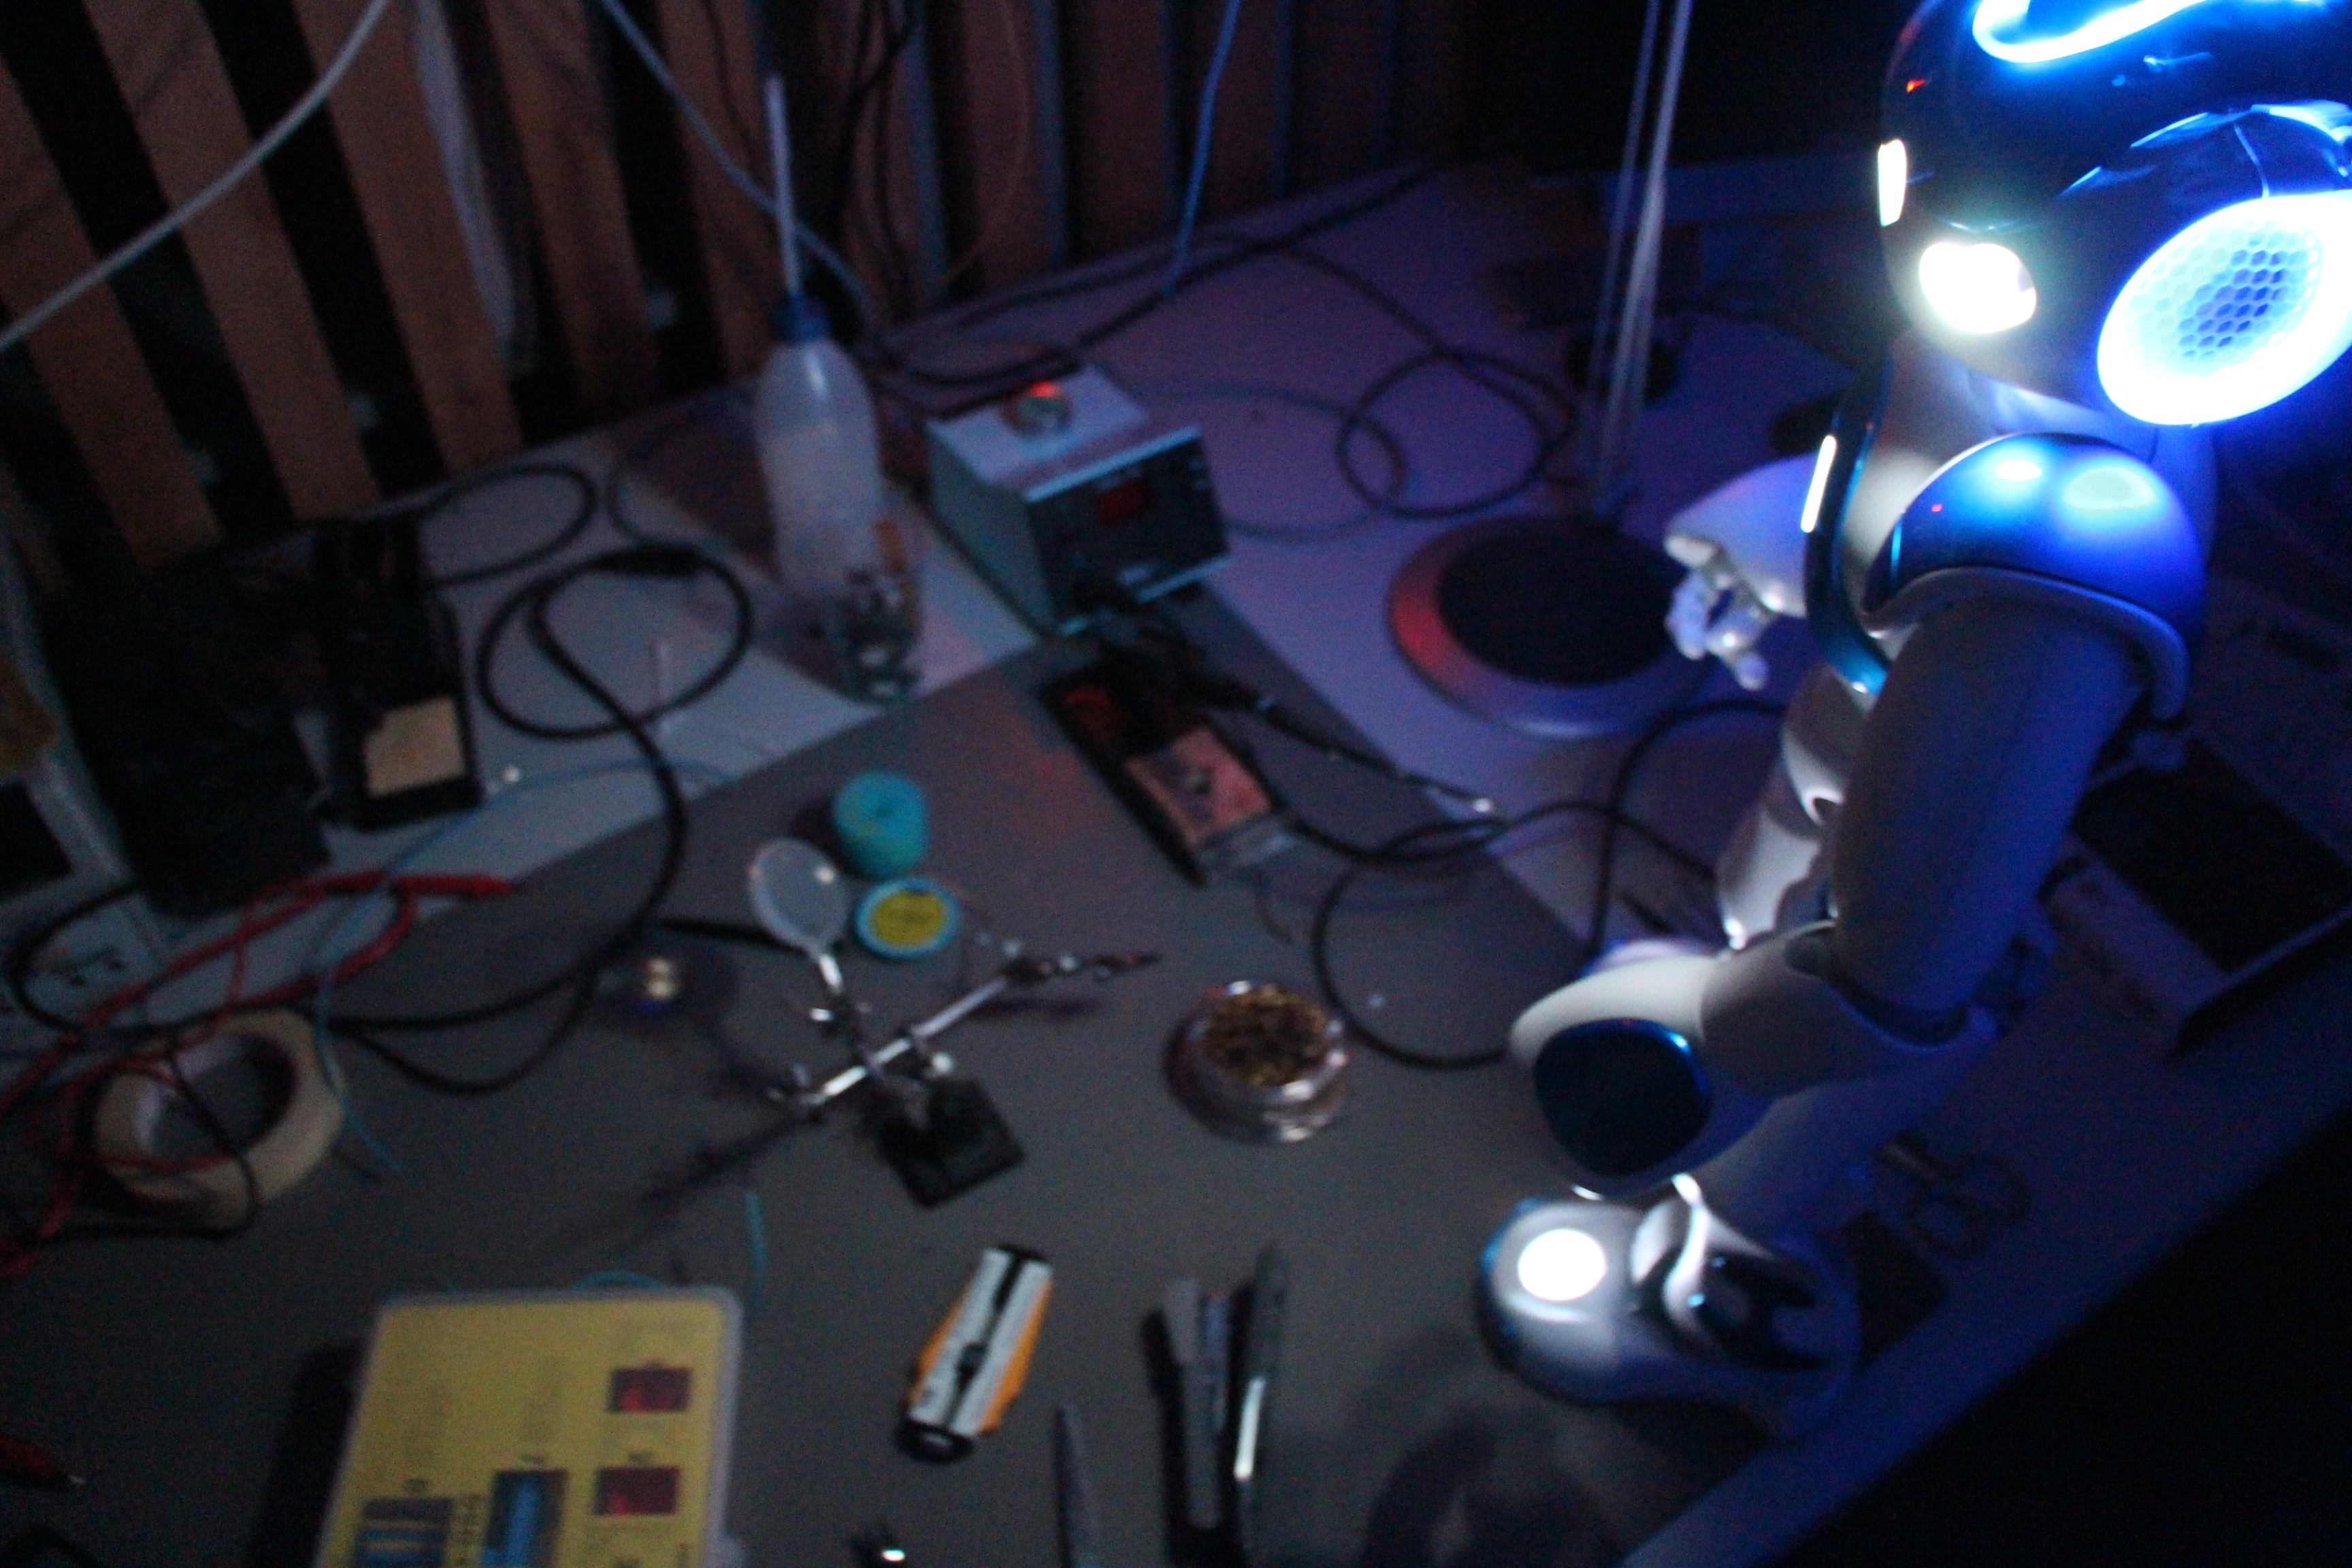
\includegraphics[width=0.9\linewidth]{mimi_mails}
%       \caption{Exemple of content of the mails sent by Mimi. A : pictures of Mimi exploring the
%           hidden base. B : some curious objects found by Mimi in the base. C :
%           few words about its adventures and discoveries.
%       }
%       \label{fig:mimi_mails}
%   \end{figure}

\begin{figure}
    \centering
    \subfigure[Initial letter, generated by the robot]{
        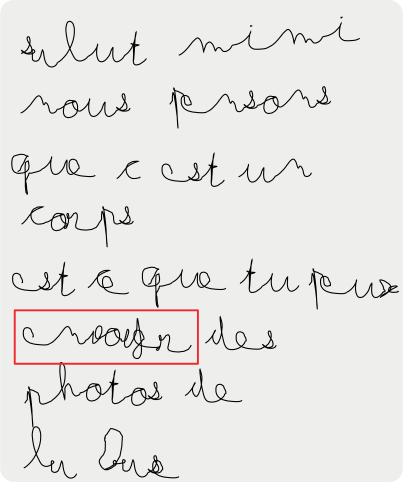
\includegraphics[height=6cm]{diego-initial-letter}
    }
    \subfigure[Final letter, after training with Vincent]{
        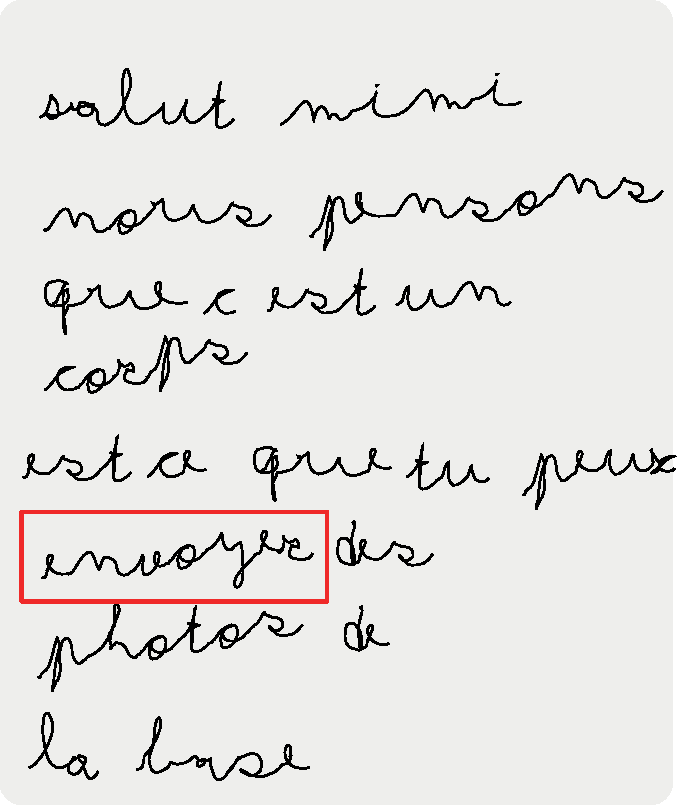
\includegraphics[height=6cm]{diego-final-letter}
    }

    \caption{\small (French) text generated by the robot, before and after a one
        hour long interaction session with the child. As an example, the red box
        highlights the changes on the word ``envoyer''.}

    \label{fig:stimuli}
\end{figure}

\begin{figure}
    \centering
    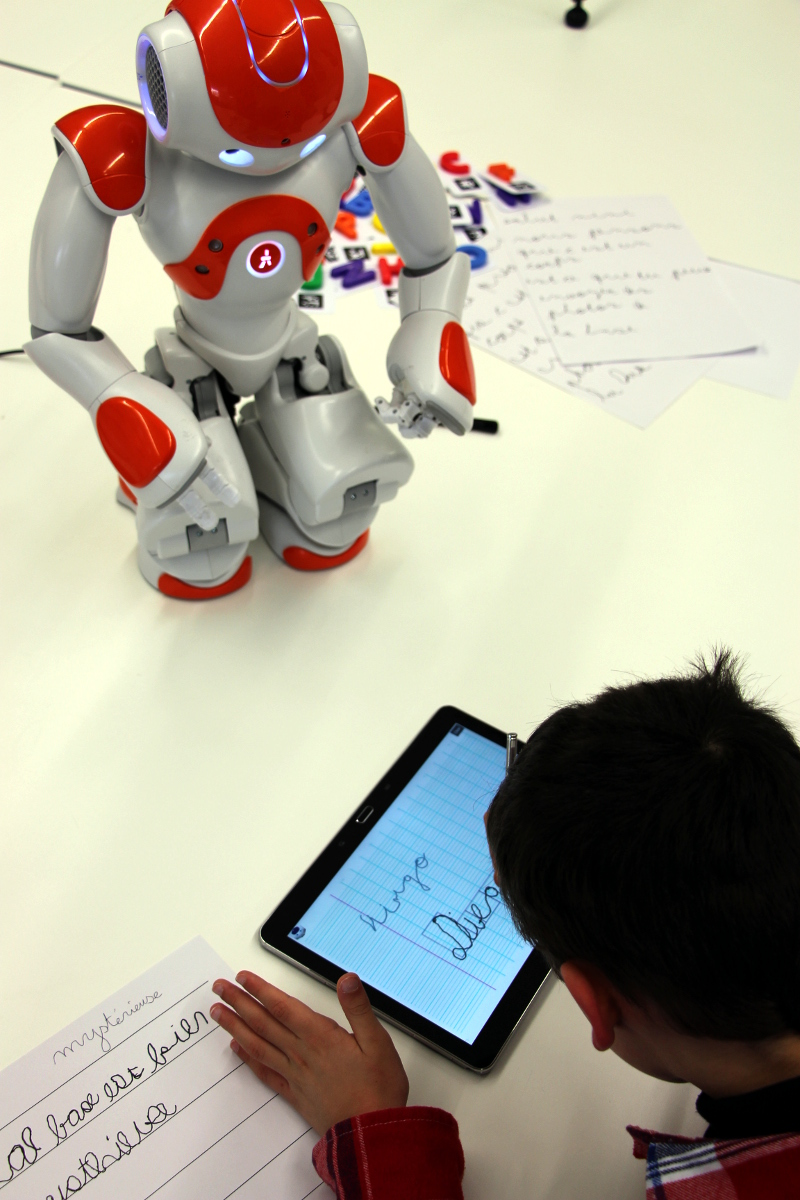
\includegraphics[width=0.5\linewidth]{diego}
    \caption{\small Vincent correcting {\sc nao}'s attempt by rewriting the
        whole word. Empty boxes are drawn on the screen to serve as template for the child
        and to make word segmentation more robust.}
    \label{fig:Vincent}
\end{figure}

\subsection{Results}
Overall, Vincent provided 154 demonstrations to the robot, and he remained
actively engaged during the four weeks. The story was well accepted and
the child seriously engaged in the game. After the first week, he showed
confidence when playing with his ``prot\'eg\'e" and he built affective bonds with the robot
over the course of the study, as evidenced by some cries on the last session,
and several letters sent to the robot \emph{after} the end of the study
(one of them 4 months later) to get news. This represents a promising initial
result: we can effectively keep a child engaged with the robot for a relatively
long periods of time (about 5 hours).

No conclusion can be drawn in terms of actual handwriting remediation: we did
not design this study to formally assess possible improvements. However, as pictured on Figure~\ref{fig:stimuli}, Vincent was able to
significantly improve the robot's skill, and he acknowledged that he had been
able to help the robot: in that regard, Vincent convinced himself that he was
``good enough'' at writing to help someone else, which is likely to have
a positive impact on his self-esteem.



\section{case study 2 : Thomas}\label{Thomas}

\subsection{Context}

Thomas, 5.5 years old child, is under the care of an occupational
therapist. He has been diagnosed with visuo-constructive deficits.
He was frequently performing random attempts and then was comparing
with the provided template. Thomas is restless and careless: he
rarely pays attention to
advice, even to what he is doing when he is currently drawing, and he is
quickly shifting his attention from one activity to another.

Thomas was working on number allographs with his therapist. During a prior
meeting, the therapist provided us with a sequence of numbers
written by Thomas. one of the observed problems was drawing
horizontally-inverted allographs, mainly for ``5".

\subsection{Questions}
This study focuses on technical adaptations of the CoWriter activity for a 
child diagnosed with writing deficits.
Our objective is to investigate small modifications of the activity adapted to
Thomas problems (visuo-constructive deficits and inattention) in order to
keep him focused
on the activity during forty-minutes sessions, and to evidence to the child that the robot is progressing by dint of his demonstrations. 

\subsection{Experimental settings}
The experiment was conducted in the therapist's office (four sessions 
spanning over 5 weeks). We assumed that a scenario like the one we used 
for Vincent would not be usable with Thomas. We just introduced the robot 
and quickly said that it was seeking help to train for a robot handwriting contest.

In order to integrate our work with that of the therapist, we decided to adapt the 
CoWriter activity to work with numbers.

Since Thomas was frequently drawing horizontally-inverted numbers, or even
unrecognisable allographs, the learning algorithm of the robot was converging to
meaningless scrawls. To fix this problem, we programmed the robot to refuse allographs that
were too distant to a reference with a threshold we arbitrary fixed. In that way,
the child was forced to take care on what he was providing to the robot as
demonstration. 

According to the therapist, it was easier for Thomas to memorize the way to draw
a number if it was always done is the same order, \emph{e.g.} if the ``5" was always
drawn from the top-right tip down to bottom. Therefore we programmed the robot to
refuse as well a good allograph drawn in a wrong order. But in order to reassure Thomas
about the right final allograph's shape, we made the robot able to recognize
such a drawing, and, when it occurred, to use the phrase:
\emph{``Oh, this is exactly the shape of the number I want to learn, but can you
show me how to draw it in the opposite direction?"}

Also, to make
the robot's progresses evident, we modified the initialization step of the
learning algorithm to start with a roughly vertical stroke instead of a
deformed number (round 0 on Figure~\ref{learning_6_demos}).

In this setup, we added a second tablet with one button per number. It was used
by the child to chose a new number to teach to the robot. It also provided the
possibility to enter letters or words, and to switch to another activity (robot telling a story if the child needs a short break).

\begin{figure}
    \centering
    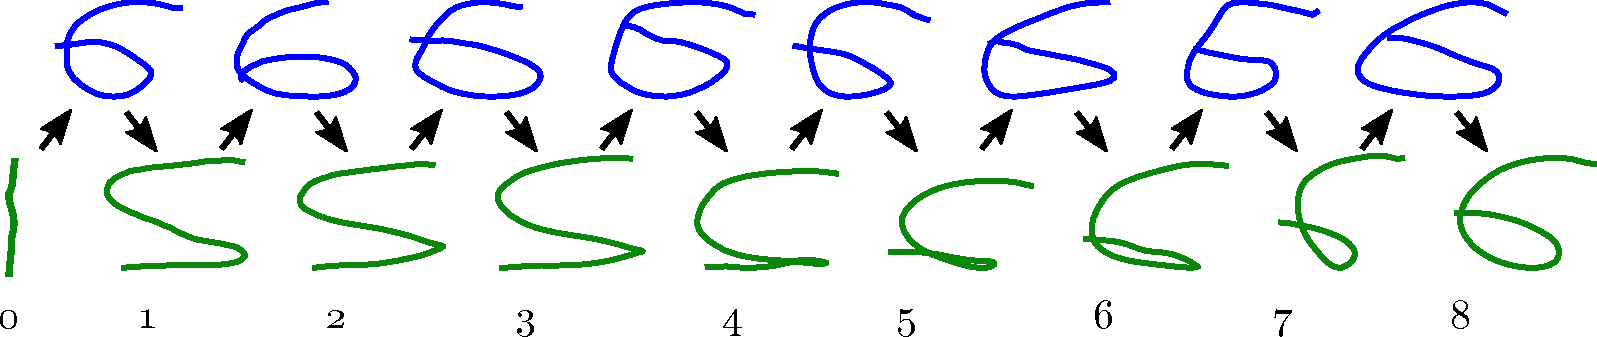
\includegraphics[width=0.9\linewidth]{learning_6_demos}
    \caption{\small Demonstrations provided by Thomas for the number ``6'' (top row) and
        corresponding shapes generated by the robot. After eight demonstrations,
        Thomas decided that the robot's ``6'' was good enough, and went to
    another character: in that respect, he was the one leading the learning
process of the robot.}
    \label{learning_6_demos}
\end{figure}

\subsection{Results}
Despite his attention deficit, Thomas was able to remain engaged in the activity during more than
forty minutes in each session. In total, 55 allographs out of 82 
demonstrated by the child were acceptable considering our threshold (with a
progressive improvement from 13 out of 28 in the first session up to 26 out
of 29 in the last session).

As soon as Thomas understood that the robot was only accepting well-formed
allographs, he started to focus on it and he would typically draw 5 or 6 times
the number before actually sending to the robot (the tablet lets children
clear their drawing and try again before sending it). According to
the therapist, it was the first time that Thomas would correct himself in such a
way, explicitly having to reflect on how \emph{another agent} (the robot) would
interpret and understand his writing. Figure~\ref{Thomas_progress} shows how
he gradually improved his demonstrations for some numbers, according to the
metric we used to make the robot accept/refuse samples.

Since the robot's handwriting started from a simple primitive (a stroke), each
time Thomas succeeded to have his demonstration accepted by it, the robot's
improvement was clearly visible (as measured in Figure~\ref{Thomas_distances}).
This led to a self-rewarding situation that effectively supported Thomas'
engagement.

\begin{figure}
    \centering
    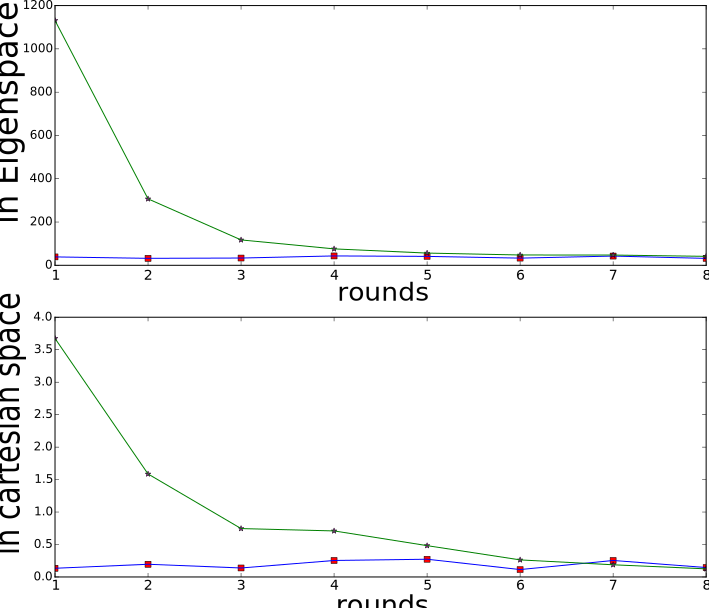
\includegraphics[width=0.9\linewidth]{learning_6_distances}
    \caption{\small Two metrics to assess the handwriting progresses: Euclidean
    distance in the subspace of the number dataset (top figure) or in
Cartesian space (bottom figure). Green lines represent the robot performance,
blue lines performance of the child. The round IDs correspond to the demonstrations
pictured on Figure~\ref{Thomas_demos}.}
    \label{Thomas_distances}
\end{figure}

%\begin{figure}
%    \centering
%    \includegraphics[width=0.9\linewidth]{learning_6_progress}
%    \caption{\small .}
%    \label{Thomas_progress}
%\end{figure}

\begin{figure}
    \centering
    \subfigure[number 1]{
        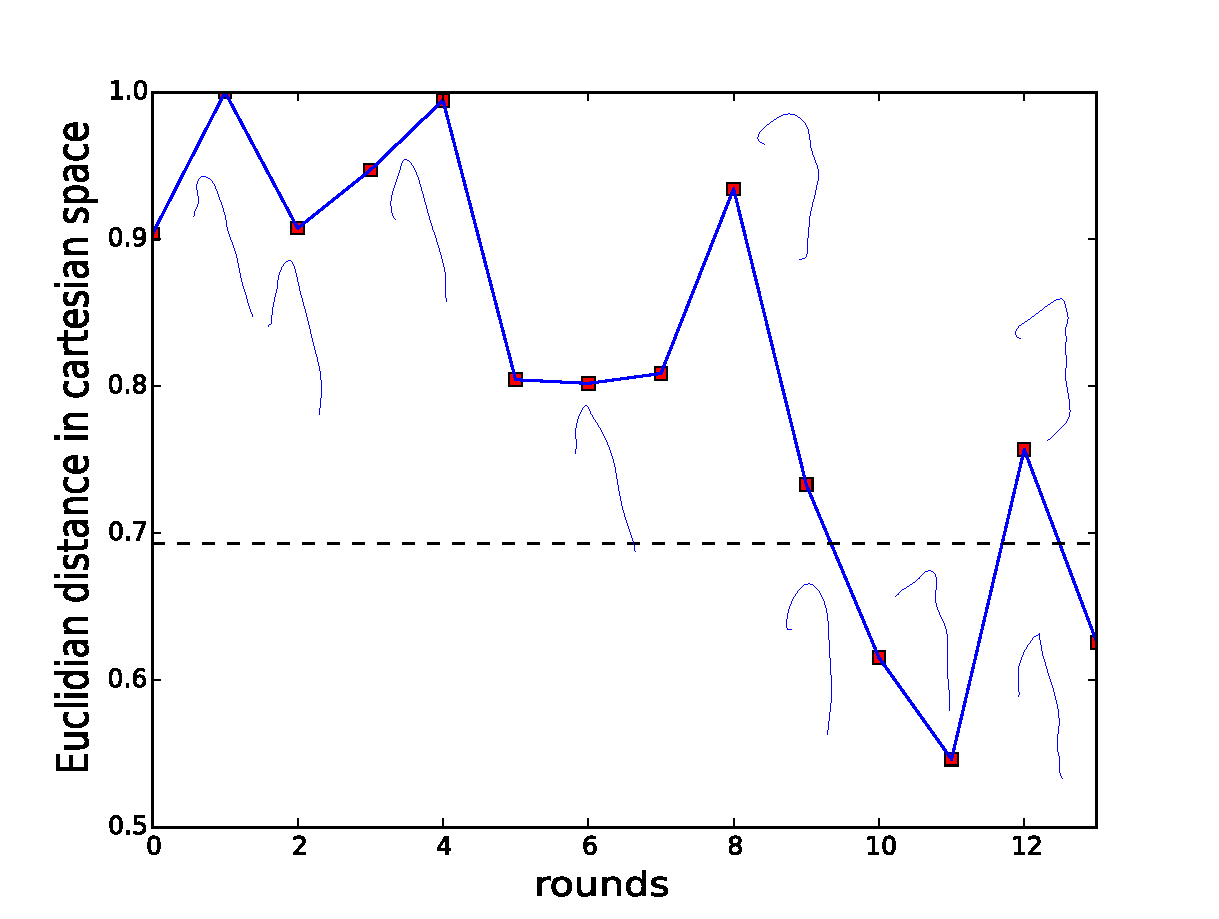
\includegraphics[width=6cm]{henry1}
    }
    \subfigure[number 2]{
        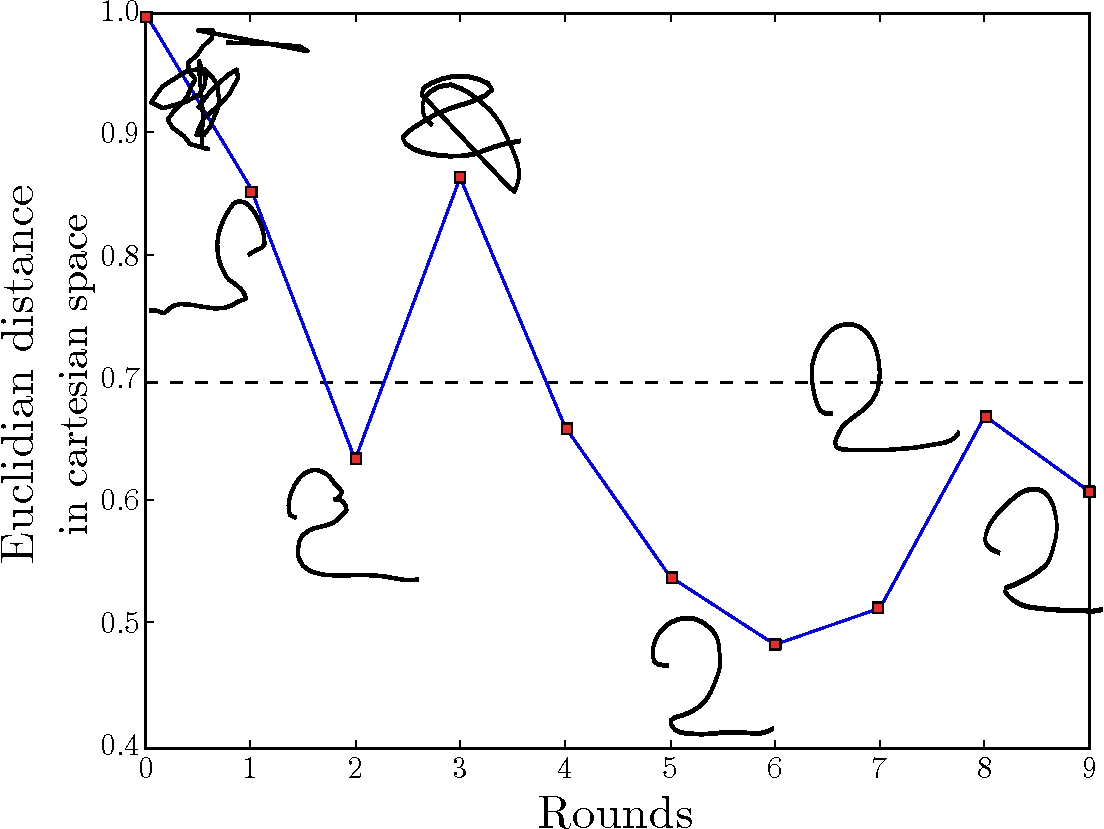
\includegraphics[width=6cm]{henry2}
    }
	\subfigure[number 5]{
        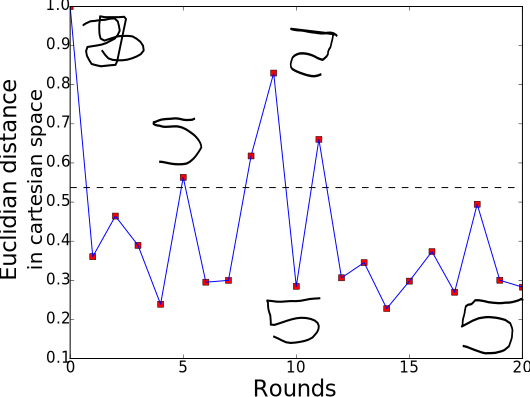
\includegraphics[width=6cm]{henry5}
    }
    \caption{\small Improvement of Thomas demonstrations for some numbers: a) drawing the allograph of the number 1, b) the number 2 and c) the number 5. Thomas progressively took care of the demonstrations he was providing to the robot for those numbers. We used for this figure the same metric than the one used for the acceptance algorithm. Distances are normalized with respect to the biggest value. The dashed line correspond to the threshold of robot's acceptance.}

    \label{Thomas_progress}
\end{figure}

\section{Case study 3: when children evaluate the robot}\label{auto}

\subsection{Context}

Each of previous studies was adapted to individual subjects : we used a special
design for each case in order to sustain the child's engagement.
In our next experiment, we conducted case studies with eight children using a single
design. Those children have in common difficulties to learn
cursive writing but the natures and intensities of those troubles are radically
different from one child to another. Valentine (7 years old), Alexandre (6.5) and
Jonathan (7) are under the care of an
occupational therapist. Enzo (8) and Matenzo (7) are repeating their school year
because of writing. Mona (6) and Adele (8) are bottom of their respective
classes in writing activities. Nathan (7) is under the care of a neurologist, and
has been diagnosed with specific language impairment. All of those children are
expected, given their school level, to know the allographs of
cursive letters. 

\subsection{Questions}

The main purpose of this study is to test the ergonomic aspects of CoWriter. When introducing the robot, we did not
provide scenario and gave to children minimal explanations. We then observed how easily children assumed the role of the teacher and how seriously they tried to help the robot.

\subsection{Experimental settings}

This experiment took place in the coffee room of a therapists shared surgery
in Normandy, France. Over two weeks, each child came three time for one-hour
session, except Adele and Mona who did just one session. A facilitator was present to explain the rules of the game and tablet usage. As in the previous experiment, children were provided with two tablets : one to choose a word (or a single letter) to teach, and one
used by both the child and the robot to write. We also provided the allograph's template if the child asked for. 

The starting point of the robot's writing was the same for all children: we
used middle point between simple vertical strokes and letters. For this study,
we wanted the robot to be only influenced by the demonstrations provided by the
child, so we did not project allographs in a subspace. The new generated
sample by the robot were calculated as the middle way between demonstration and
last state in Cartesian space. 

The robot was programmed to accept all demonstrations, giving to the child the
full responsibility of the teacher.

We added two buttons on the tablet  interface: a green one with a ``thumbs up", and
a red one with a ``thumbs down". Those buttons could be used by children to evaluate the
robot (the green one was for rewards while the red one was for punishment). This
way, we could measure the perception of the robot by the child: the more the
child used evaluation buttons, the more he was playing the teacher, judging the
robot instead of himself. It became possible to estimate if a child is playing
seriously given correlation between his evaluation and robot's actual
progression.


\subsection{Results}

All children maintained their engagement during the whole sessions. They provided
on average 42 demonstrations per session. All children used evaluation buttons and
had preference to reward the robot (in total, 99 rewards and 33 punishments were recorded). 

Since sessions took place over only two weeks, we did not studied possible
handwriting remediation in children, but we focused on correlation between the children's evaluations and the robot's progression.
We estimated the robot's progression as the difference between a starting score
(score of the first robot's try when children have chosen a new word/letter to
work on) and the current robot's score (after being taught by the child). The
score is calculated as the average of euclidean
distance between robot's try and a reference allograph over all letters of the
word. Those references for letter allographs where drawn by us beforehand, taking inspiration in education.com cursive letters template\footnote{\url{http://www.education.com/slideshow/cursive-handwriting-z/}}. Let $P_i$ be the
estimated progression of the robot at time $ i$. Of course, if the child
chose to switch to a new word at time $ j$ , we have $ P_{j}=0$ and clearly $
P_0=0$.
To measure whether the fact that the child was rewarding the robot when it was
progressing was significant or not, we generated 10000 times the same number of reward/punishment
but accorded at random times. Let $ R_i^n$ be the $n^{th}$ generated evaluation at
time $ i$ ($ R_i^n = 0$ if
no evaluation occurred at time $ i$ , $ R_i^n=1$ if a reward occurred at time
$i$ and $R_i^n=-1$ if a punishment occurred at time $i$), and $\overline{R}_i$ be the
actual evaluation at time $i$. For each $n^{th}$ generated sequence of evaluation, we
compute a score of evaluation: $$ S^n = \sum\limits_i{R_i^n P_i}$$ 
Then we can estimate the p-value $p$ of the actual score: $$ \overline{S} =
\sum\limits_i{\overline{R}_i P_i}$$ 
given the distribution of the generated scores $\left(S^n\right)_n$, which is assumed to
be Gaussian: 
$$p(\overline{S})= \mathbb{P}{\left[X>\overline{S}\right]} = 1-\phi{\left(\frac{\overline{S}-\mu}{\sigma}\right)}$$
where $\phi$ denotes the cumulative distribution function of the standard normal
distribution, $\mu$ the mean and $\sigma$ the deviation of the generated 
scores $\left(S^n\right)_n$. 
As a result, we found that 5 of the 8 children obtained a score of evaluation
significantly hight ($p(\overline{S})<0.05$). Score of evaluation
p-values of each child is reported in the second-to-last column of Table~\ref{table:scores}.

We also studied correlation between children's evaluations and their own
progression. The analysis was conducted in the same way, using distances between children
demonstrations and reference allographs to compute children progressions.
3 of 5 children that played ``seriously" obtained score of evaluation of their own
progression significantly high (last column of Table~\ref{table:scores}). For
those children, it seems that the robot was reflecting their own performances, and while they
were judging the robot positively (three times more rewards than punishments)
they were actually evaluating themselves.




\begin{table}
    \centering
    \begin{tabular}{|c|c|c|c|c|c|}
        \hline
        child & demo & rew & pun & p(robot) & p(child)\\ \hline
        valentine & 127 & 24 & 6 & 2.4e-03 & 5.5e-02\\ \hline
        enzo & 223 & 20 & 9 & 1.7e-01 & 3.5e-01\\ \hline
        matenzo & 131 & 10 & 3 & 3.8e-03 & 7.9e-03\\ \hline
        jonathan & 98 & 10 & 5 &  1.5e-01 & 3.8e-01\\ \hline
        nathan & 115 & 16 & 4 & 5.3e-04 & 2.7e-03\\ \hline
        alexandre & 83 & 10 & 3 & 3.1e-02 & 6.0e-01\\ \hline
        adele & 35 & 4 & 2 & 5.0e-02 & 3.7e-02\\ \hline
        mona & 40 & 5 & 1 &  5.4e-01 & 2.0e-01\\ \hline
    \end{tabular}
    \caption{\small results of evaluations. demo: number of demonstrations provided by
        the child over all session. rew: number of rewards accorded by
        the child. pun: number of punishments. p(robot): are the evaluations
        significantly corresponding to the progression of the robot ? p(child): are the
        evaluations significantly corresponding to the child's own
progression ?}
    \label{table:scores}
\end{table}


\section{Conclusion}
This paper provides the first results of long-term experiments 
with CoWriter activity performed by one child at the time. 

We introduced some adaptations of
the interaction design and the learning algorithm that succeeded in keeping
children engaged during repetitive long sessions ($\thicksim$ 45 minutes, 3 or 4 times).
These designs of long-term interactions provide
opportunities for studying and improving actual impact of human-robot activities as
education tools.

The fact that a child with real difficulties in handwriting can easily
understand the activity and feel that the robot actually learns from his
demonstrations reveals that CoWriter could have a positive therapeutic impact.

The evaluation of the robot by the child provided information about his
understanding of the activity and how much he was satisfied with the
learning process (both the robot's ability to learn and the child's own
ability to teach). We believe that this information could be taken into account by
the robot in order to improve the quality of the interaction. As an example, it
could be used at two levels: $\bullet$ it is possible to detect if the child is playing
seriously or not (a non-serious child may provide unrecognisable drawings and gives good grades to
the robot while its level decreases), or if the child did not understand the
activity (if he never uses the evaluation buttons and spends a lot of time to
give a response). $\bullet$ We can reinforce the learnt allograph when the robot
receives a good evaluation, or make it forget the allograph when it
receives a bad evaluation.

After all those
experiments, we now have a large database of children writings that could be
used to generate more interesting subspaces by PCA and robot initial states. 
Recurrent neural networks (RNN) for handwriting recognition and generation~\cite{DBLP:journals/corr/Graves13} could also be used to generate 
children-like handwriting.

\section*{Acknowledgments}

This research was partially supported by the Funda\c{c}\~{a}o para a Ci\^{e}ncia
e a Tecnologia (FCT) with reference UID/CEC/ 50021/2013, and by the Swiss
National Science Foundation through the National Centre of Competence in
Research Robotics.

\bibliographystyle{abbrv}

\bibliography{cowriter} 

\end{document}
